\title{Computer Networks - CS 204} % You may change the title if you want.

\author{Rishit Saiya - 180010027, Assignment - 4}

\date{\today}

\documentclass[12pt]{article}
\usepackage{fullpage}
\usepackage{enumitem}
\usepackage{amsmath,mathtools}
\usepackage{amssymb}
\usepackage[super]{nth}
\usepackage{multirow}
\usepackage[normalem]{ulem}
\useunder{\uline}{\ul}{}
\usepackage{textcomp}
\usepackage{calc}
\usepackage{tikz}
\usepackage{hyperref}
        
\begin{document}
\maketitle

%---------------------------------------------------------------------

\section{}

We use the idea of Conservation of Data with the factor of transmission keeping in mind. The required data rate (D) is as follows:
\begin{equation*}
    D = N \times 1000 \, \frac{bits}{packet} \times \frac{1}{100} \, \frac{packet}{seconds}
\end{equation*}
or,
\begin{equation*}
    D = 10 \times N \, \frac{bits}{second}    
\end{equation*}
With the reference to the literature, we know that using the implementation of Unslotted/Pure ALOHA, the available data rate is 18\% of 56,000 $\frac{bits}{second}$.
Hence, finally equating both,
\begin{equation*}
    10 \times N \, \frac{bits}{second} = 0.18 \times 56,000\, \frac{bits}{second}
\end{equation*}
or,
\begin{equation*}
    N = 1008
\end{equation*}
It is to be noted that, we used 18\% for the pure ALOHA (which is maximum possible), so the resulting N is also maximum value.

%-------------------------------------------------------------------

\section{}

With pure ALOHA, transmission can be started immediately whereas with the slotted ALOHA, transmission has to wait to the next slot.

%-------------------------------------------------------------------

\section{}

Given that, the efficiency of slotted ALOHA is Np$(1-p)^{(N-1)}$, where N is the number of Active nodes and the p is the probability of transmission.

Let us assume the Efficiency to be E.
\begin{equation*}
    E = Np(1-p)^{N-1}
\end{equation*}
We see that, efficiency is dependent upon the parameter p, so in order to find the maximum efficiency, we need to derive the value of p such that E will be maximum.
We do the following:
\begin{equation*}
    \frac{dE}{dp} = 0
\end{equation*} 
\begin{equation*}
    (1-p)^{N-1} - p(N-1)(1-p)^{N-2} = 0
\end{equation*}
\begin{equation*}
    1-p = p \times (N-1)
\end{equation*}
or,
\begin{equation*}
    p = \frac{1}{N}    
\end{equation*}

Maximum E is attained at E(p = $\frac{1}{N}$).
\begin{equation*}
    E = (1 - \frac{1}{N})^{N-1}
\end{equation*}

As N approaches $\infty$, we calculate E there. 
\begin{equation*}
    E_{max} = \lim_{N \to \infty} E
\end{equation*}
\begin{equation*}
    E_{max} = \lim_{N \to \infty} (1 - \frac{1}{N})^{N-1}
\end{equation*}
\begin{equation*}
    E_{max} = \exp (\lim_{N \to \infty}(1 - \frac{1}{N} - 1) \times (N-1))
\end{equation*}
\begin{equation*}
    E_{max} = 1/e
\end{equation*}

%-------------------------------------------------------------------

\section{}
For pure ALOHA, we follow the similar process as above. Here the Efficiency is given as follows:
\begin{equation*}
    E = Np(1-p)^{2(N-1)}
\end{equation*}

We see that, efficiency is dependent upon the parameter p, so in order to find the maximum efficiency, we need to derive the value of p such that E will be maximum.
We do the following:
\begin{equation*}
    \frac{dE}{dp} = 0
\end{equation*} 
\begin{equation*}
    (1-p)^{2(N-1)} - p(2(N-1))(1-p)^{2(N-1)-1} = 0
\end{equation*}
\begin{equation*}
    1-p = p \times (2N-2)
\end{equation*}
or,
\begin{equation*}
    p = \frac{1}{2N-1}    
\end{equation*}

Maximum E is attained at E(p = $\frac{1}{2N-1}$).
\begin{equation*}
    E = N(\frac{1}{2N-1})(1 - \frac{1}{2N-1})^{2(N-1)}
\end{equation*}

As N approaches $\infty$, we calculate E there. 
\begin{equation*}
    E_{max} = \lim_{N \to \infty} E
\end{equation*}
\begin{equation*}
    E_{max} = \lim_{N \to \infty} N(\frac{1}{2N-1})(1 - \frac{1}{2N-1})^{2(N-1)}
\end{equation*}
\begin{equation*}
    E_{max} = \frac{1}{2} \times \exp (\lim_{N \to \infty}(1 - \frac{1}{2N-1} - 1) \times 2(N-1))
\end{equation*}
\begin{equation*}
    E_{max} = 1/2e
\end{equation*}
%-------------------------------------------------------------------

\section{}
%Graphs to be put here.
The graphs are as follows: \\

The efficiencies of Slotted and Pure ALOHA for N=15, is given in Figure 1.
\begin{figure}
    \centering
    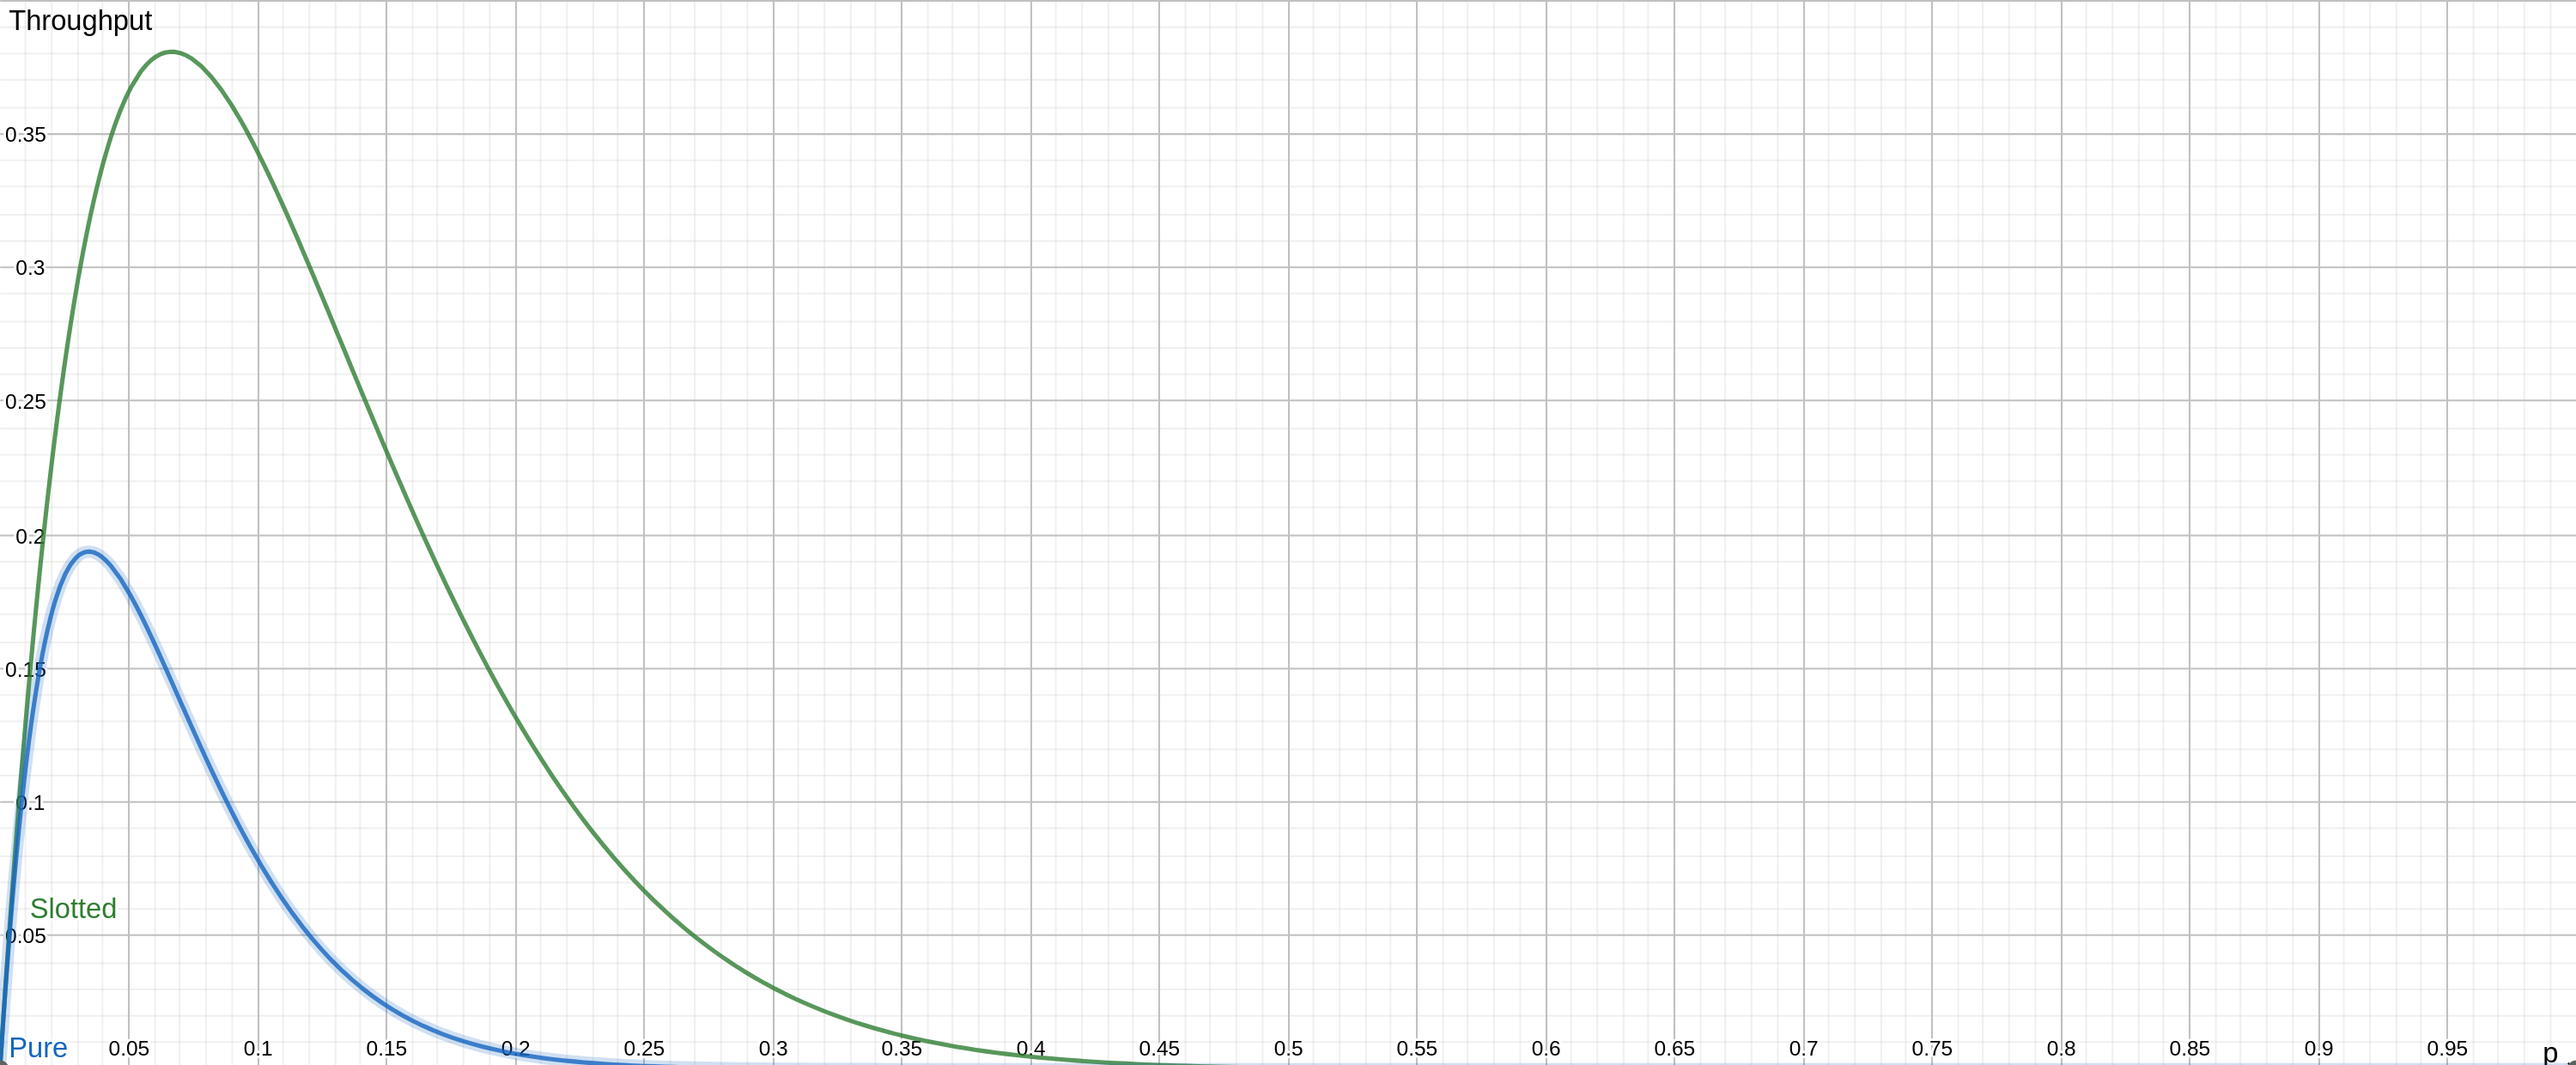
\includegraphics[width=10cm, height=5cm]{N_15.png}
    \caption{Pure ALOHA vs. Slotted ALOHA, N=15}
\end{figure}

The efficiencies of Slotted and Pure ALOHA for N=25, is given in Figure 2.
\begin{figure}
    \centering
    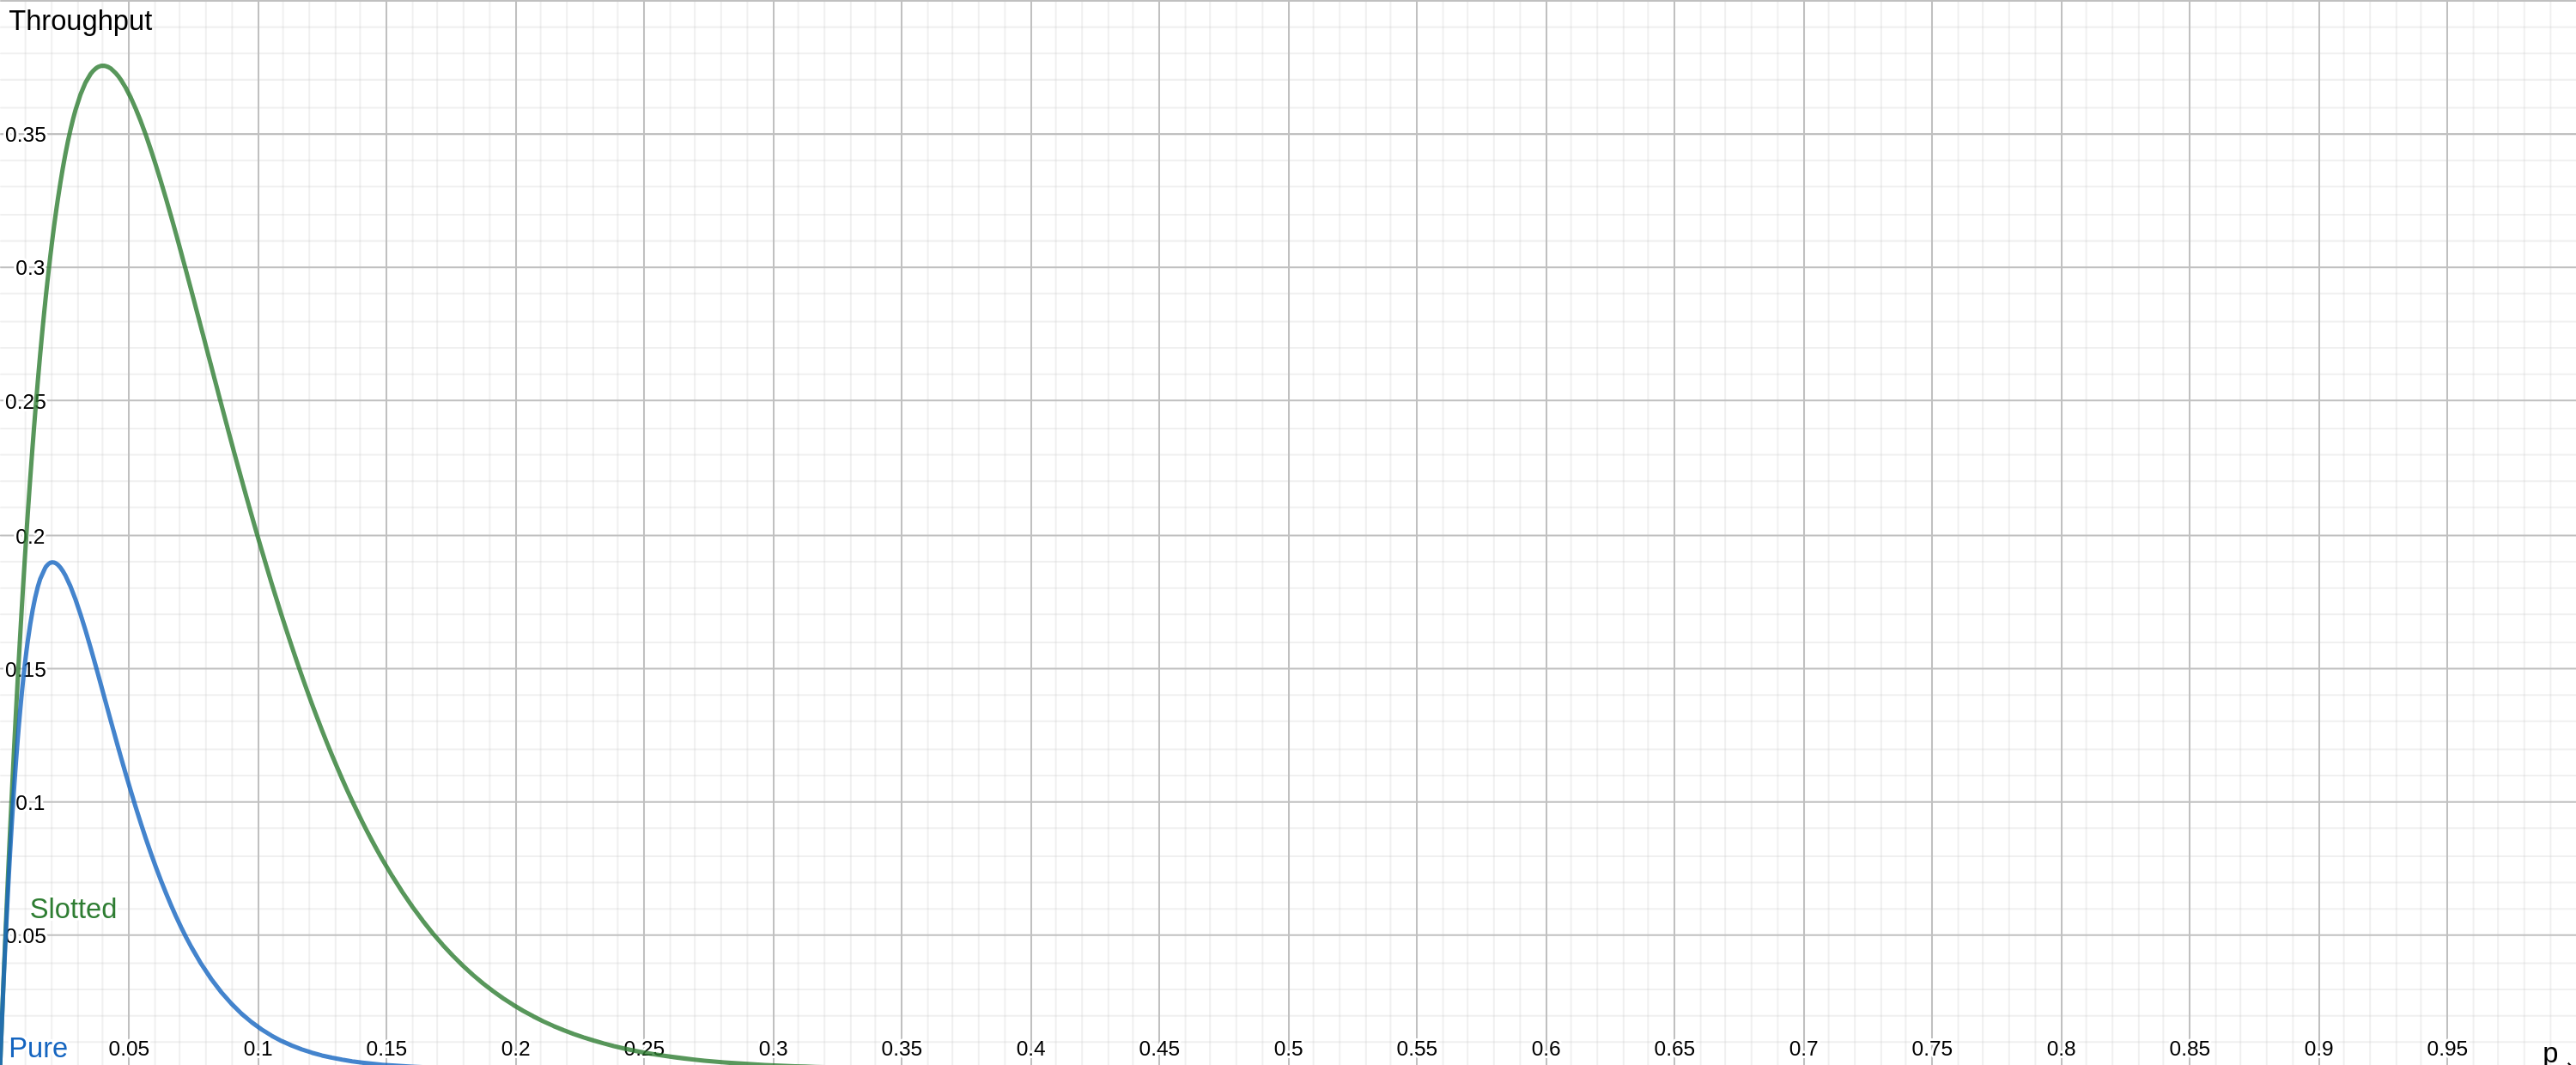
\includegraphics[width=10cm, height=5cm]{N_25.png}
    \caption{Pure ALOHA vs. Slotted ALOHA, N=25}
\end{figure}

The efficiencies of Slotted and Pure ALOHA for N=35, is given in Figure 3.
\begin{figure}
    \centering
    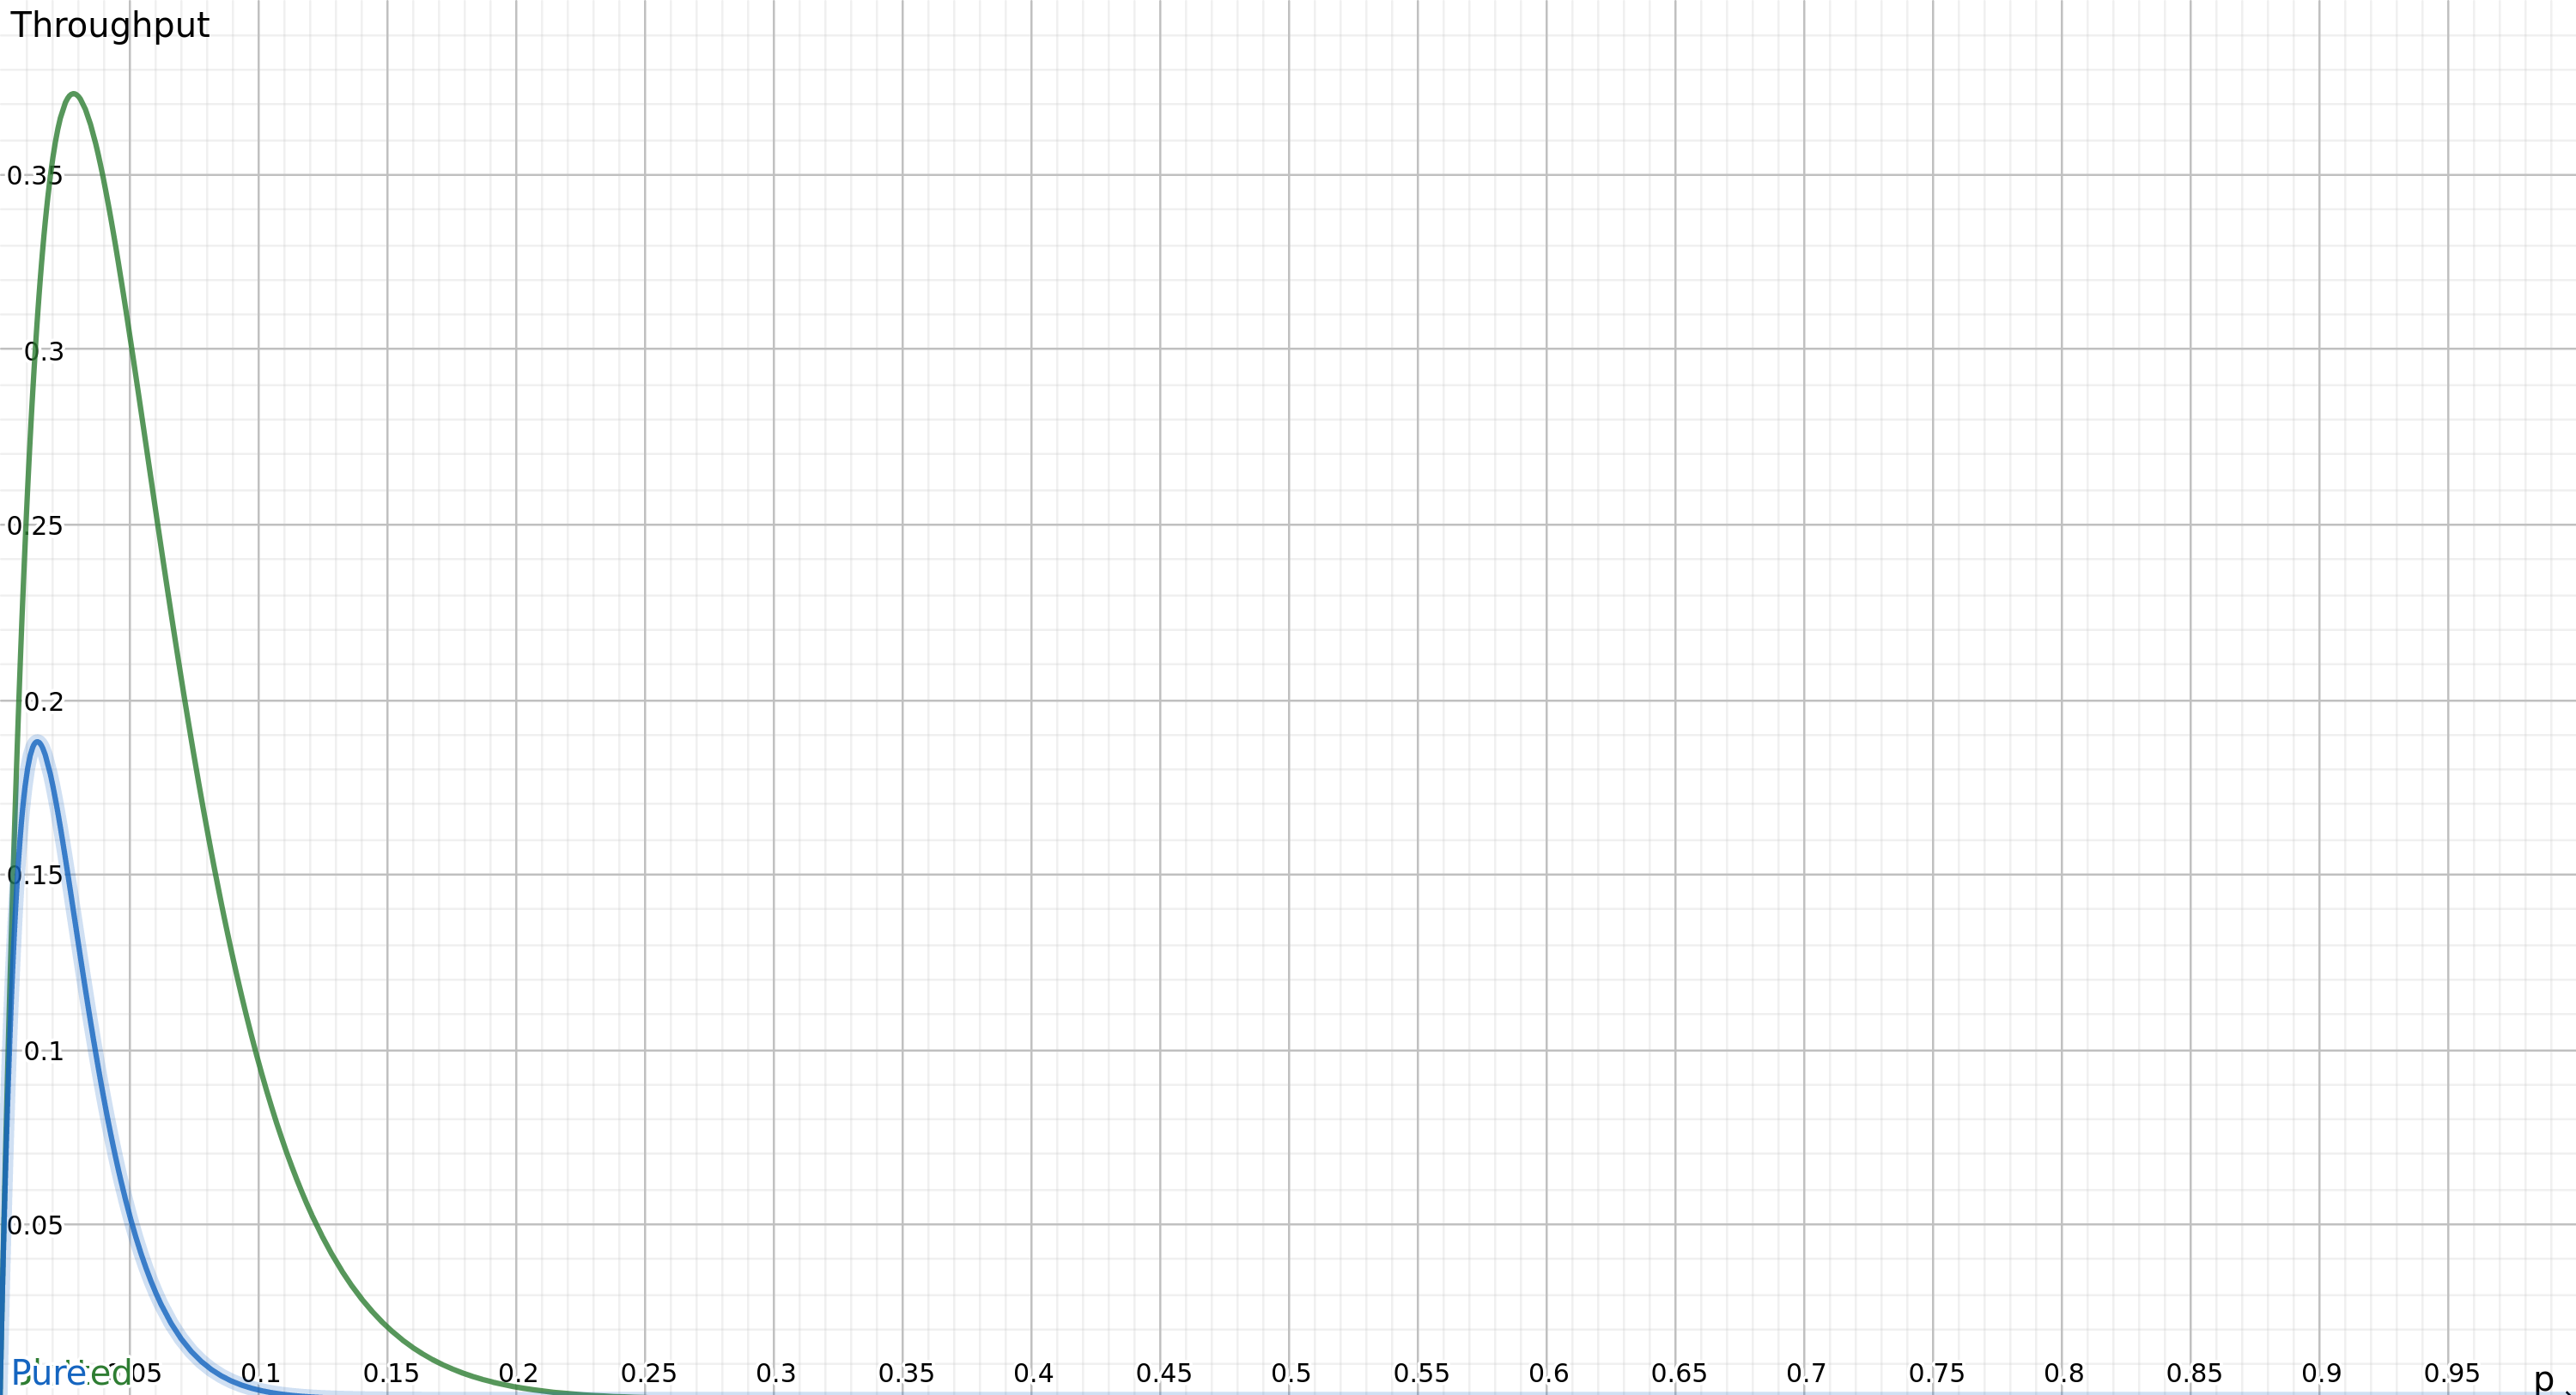
\includegraphics[width=10cm, height=5cm]{N_35.png}
    \caption{Pure ALOHA vs. Slotted ALOHA, N=35}
\end{figure}


For all given N, Slotted ALOHA gives higher efficiency than the Pure ALOHA. Furthermore, we observe that as the value of N increases, the graph becomes narrower. As the N is increasing, the area under the curves decreases but still it is to be noted that efficiencies remain constant irrespective of the values of N.
%--------------------------------------------------------------------

\section{}
In accordance with the Binary Exponential Backoff Algorithm, if the node is chosen after $5^{th}$ collision, then K is chosen from the set \{0,1,2,...$2^5-1$\} and the corresponding delay would be K $\times$ 51.2 $\mu$sec.

\begin{equation*}
    P(K = 4) = \frac{1}{32}
\end{equation*}
Where P is the probability that a node chooses K = 4, after the $5^{th}$ collision in CSMA/CD. \\
To calculate the delay, we just have to do the following:
\begin{equation*}
    data_{delay} = 4 \times 512 \, bits   
\end{equation*}
or,
\begin{equation*}
    t_{delay} = \frac{4 \times 512}{10 \times 10^6} \, \frac{bits}{\frac{bits}{second}}   
\end{equation*}
\begin{equation*}
    t_{delay} = 204.8 \, \mu sec
\end{equation*}

%--------------------------------------------------------------------

\section{}

Given that G = 1001, and D = 101110, we calculate G expression for the sake of completeness which is given as follows:
\begin{equation*}
    G = 1 \times x^3 + 0 \times x^2 + 0 \times x^1 + 1 \times x^0
\end{equation*}
or,
\begin{equation*}
    G = x^3 + 1
\end{equation*}
Clearly, from above G expression, r = 3. \\
The bit pattern D+r pattern becomes 10110000.
To calculate the R, we do the following process.

Now, divide and XOR the message with divisor polynomial bits. Make resultant remainder to 5 bit again and that is the CRC send along with the message.

The R = 100 in this case.

%--------------------------------------------------------------------

\section{}

Given that G = 10011, and D = 1010101010, we calculate G expression for the sake of completeness which is given as follows:
\begin{equation*}
    G = 1 \times x^4 + 0 \times x^3 + 0 \times x^2 + 1 \times x^1 + 1 \times x^0
\end{equation*}
or,
\begin{equation*}
    G = x^4 + x + 1
\end{equation*}
Clearly, from above G expression, r = 4. \\
The bit pattern D+r pattern becomes 10101010100000.
To calculate the R, we do the following process.

Now, divide and XOR the message with divisor polynomial bits. Make resultant remainder to 5 bit again and that is the CRC send along with the message.

The R = 00100 in this case.

%--------------------------------------------------------------------

\section{}

\begin{enumerate}[label=(\alph*)]
    
    \item Clearly, from G , r = 4. \\
The bit pattern D+r pattern becomes 10010101010000.
To calculate the R, we do the following process:

Now, divide and XOR the message with divisor polynomial bits. Make resultant remainder to 5 bit again and that is the CRC send along with the message.

The R = 00000 in this case.
    
    \item Clearly, from G , r = 4. \\
The bit pattern D+r pattern becomes 01011010100000.
To calculate the R, we do the following process:

Now, divide and XOR the message with divisor polynomial bits. Make resultant remainder to 5 bit again and that is the CRC send along with the message.

The R = 01111 in this case.
    
    \item Clearly, from G , r = 4. \\
The bit pattern D+r pattern becomes 10101000000000.
To calculate the R, we do the following process:

Now, divide and XOR the message with divisor polynomial bits. Make resultant remainder to 5 bit again and that is the CRC send along with the message.

The R = 01001 in this case.
\end{enumerate}

%----------------------------------------------------------------------

\section{}

2-D Parity is the generalization of the simple 1-D parity scheme using the following steps:

\begin{enumerate}
    \item Generate a M $\times$ N matrix of bits.
    \item Add a (even or odd) parity bit to each row and to each column depending upon the parity scheme chosen.
\end{enumerate}

Since we are using an even parity scheme, we obtain the matrix as given in Table 1.

\begin{table}[]
\begin{center}
\begin{tabular}{|c|c|c|c|c|c|}
\hline
\multicolumn{1}{|l|}{}                & \multicolumn{4}{c|}{\textbf{Bit Pattern}}         & \textbf{Parity Bits} \\ \hline
\multirow{4}{*}{\textbf{Bit Pattern}} & 1          & 1          & 1          & 0          & \textbf{1}           \\ \cline{2-6} 
                                      & 0          & 1          & 1          & 0          & \textbf{0}           \\ \cline{2-6} 
                                      & 1          & 0          & 0          & 1          & \textbf{0}           \\ \cline{2-6} 
                                      & 1          & 1          & 0          & 1          & \textbf{1}           \\ \hline
\textbf{Parity Bits}                  & \textbf{1} & \textbf{1} & \textbf{0} & \textbf{0} & \textbf{0}           \\ \hline
\end{tabular}
\caption{Fields of 2-D Even Parity Scheme for the given Bit Pattern}
\end{center}
\end{table}

%----------------------------------------------------------------------

\section{}

Consider a case, where the sent bit pattern is as given in Table 2. Now consider that the received bit pattern is as given in Table 3.

\begin{table}[]
\begin{center}
\begin{tabular}{|c|c|c|c|c|c|}
\hline
\multicolumn{1}{|l|}{}                & \multicolumn{4}{c|}{\textbf{Bit Pattern}}         & \textbf{Parity Bits} \\ \hline
\multirow{4}{*}{\textbf{Bit Pattern}} & 1          & 1          & 1          & 0          & \textbf{1}           \\ \cline{2-6} 
                                      & 0          & 1          & 1          & 0          & \textbf{0}           \\ \cline{2-6} 
                                      & 1          & 0          & 0          & 1          & \textbf{0}           \\ \cline{2-6} 
                                      & 1          & 1          & 0          & 1          & \textbf{1}           \\ \hline
\textbf{Parity Bits}                  & \textbf{1} & \textbf{1} & \textbf{0} & \textbf{0} & \textbf{0}           \\ \hline
\end{tabular}
\caption{Sender's Bit Pattern with corresponding Parity Bits}
\end{center}
\end{table}

\begin{table}[]
\begin{center}
\begin{tabular}{|c|c|c|c|c|c|}
\hline
\multicolumn{1}{|l|}{}                & \multicolumn{4}{c|}{\textbf{Bit Pattern}}                        & \textbf{Parity Bits} \\ \hline
\multirow{4}{*}{\textbf{Bit Pattern}} & 1          & 1                         & 1          & 0          & \textbf{1}           \\ \cline{2-6} 
                                      & 0          & {\ul \textit{\textbf{0}}} & 1          & 0          & \textbf{0}           \\ \cline{2-6} 
                                      & 1          & 0                         & 0          & 1          & \textbf{0}           \\ \cline{2-6} 
                                      & 1          & 1                         & 0          & 1          & \textbf{1}           \\ \hline
\textbf{Parity Bits}                  & \textbf{1} & \textbf{1}                & \textbf{0} & \textbf{0} & \textbf{0}           \\ \hline
\end{tabular}
\end{center}
\caption{Receiver's Bit Pattern with 1 error and corresponding Parity Bits}
\end{table}

When the receiver receives an erroneous frame with Data bits and the parity bits together, the parity bits in the frame will be the ones which were computed by the sender using the actual error-free data. So, now when the frame arrives at the receiver, it simply calculates the number of 1's in every row and every column, and then compares the same with the corresponding parity bits (at every row and every column) as sent by the sender. Whenever there is a mismatch in the number of 1s and the value of the parity bit, it knows that there is an error in that particular row/column. To be sure about the particular bit index, it further looks at the parity bit corresponding row and column, i..e, if the bit has an index (i,j), then for error to happen at that index, the corresponding row as well as column parity as computed by the receiver will be different from the parity bits sent by the sender.

As for the above example is concerned, the bit at bit\_pattern[2][2] (Underlined bit) was the error and it was detected and corrected.

Consider that Table 4 as the receiver's bit pattern with 2 errors. It has errors at bit\_pattern[2][2] $\And$ bit\_pattern[3][2].
\begin{table}[]
\begin{center}
\begin{tabular}{|c|c|c|c|c|c|}
\hline
\multicolumn{1}{|l|}{}                & \multicolumn{4}{c|}{\textbf{Bit Pattern}}                        & \textbf{Parity Bits} \\ \hline
\multirow{4}{*}{\textbf{Bit Pattern}} & 1          & 1                         & 1          & 0          & \textbf{1}           \\ \cline{2-6} 
                                      & 0          & {\ul \textit{\textbf{0}}} & 1          & 0          & \textbf{0}           \\ \cline{2-6} 
                                      & 1          & {\ul \textit{\textbf{1}}} & 0          & 1          & \textbf{0}           \\ \cline{2-6} 
                                      & 1          & 1                         & 0          & 1          & \textbf{1}           \\ \hline
\textbf{Parity Bits}                  & \textbf{1} & \textbf{1}                & \textbf{0} & \textbf{0} & \textbf{0}           \\ \hline
\end{tabular}
\end{center}
\caption{Receiver's Bit Pattern with 2 error and corresponding Parity Bits}
\end{table}

Clearly, this mechanism can detect those errors but cannot correct them.

%----------------------------------------------------------------------


\end{document}